\documentclass{beamer}

\usepackage[utf8]{inputenc}
\usepackage{fancybox}
\usepackage{environ}
\usepackage{verbatim}

\title{\mbox{2.3 Linear Equations} \\ \phantom{foo}}

%\subtitle[short version]{}

\date{%
}

\author{\mbox{Ed Bueler}}

\institute{\scriptsize Dept.~of Mathematics and Statistics \\ UAF}

\usetheme{Pittsburgh}

\setbeamercolor{normal text}{fg=white,bg=black}

\NewEnviron{rightframe}[1][]{%
\begin{frame}[t]
\frametitle{#1}
\begin{columns}
\begin{column}{0.4\textwidth}
%nothing
\end{column}
\begin{column}{0.6\textwidth}
\BODY
\end{column}
\end{columns}
\end{frame}
}


\begin{document}

\begin{rightframe}[]
\titlepage

\vspace{30mm}
\tiny {\color{blue!30} D. Zill, \emph{A First Course in Differential Equations with Modeling Applications}, 11th ed.}
\end{rightframe}



\begin{rightframe}[]
a \emph{linear} ordinary differential equation has a first power on both $dy/dx$ and $y$ \emph{and} it can be put in the form
        $$a_1(x) \frac{dy}{dx} + a_0(x) y = g(x)$$
or
        $$\frac{dy}{dx} + P(x) y = g(x)$$

\bigskip
\emph{main idea}:  we can write solutions to such equations in terms of integrals
\end{rightframe}

\begin{rightframe}[]
linear equation standard form:
        $$\frac{dy}{dx} + P(x) y = g(x)$$

\only<2-5>{
\begin{itemize}
\only<2>{
    \item \textbf{Example}.
        $$\frac{dy}{dx} + y = x+3$$
    Here $P(x)=1$ and $g(x) = x+3$.
}
\only<3>{
    \item \textbf{Example}.
        $$t z' = z + \cos t$$
    which is the same as
        $$\frac{dz}{dt} + \frac{-1}{t} z = \frac{\cos t}{t}$$
    with $P(t) = -1/t$ and $g(t)=\cos t/t$.
}
\only<4-5>{
    \item \textbf{Not an example}.
        $$y \frac{dy}{dx} = x+e^x$$
    this cannot be put in the standard form
    
    \only<5>{\dots but it is \emph{separable} (section 2.2)}
}
\end{itemize}
}
\end{rightframe}


\begin{rightframe}[]
before giving general formulas, here's how the method works on an example

\begin{itemize}
    \item \textbf{Example}.
        $$\frac{dy}{dx} + y = x+3$$
\end{itemize}
\end{rightframe}


\begin{rightframe}[]
to solve a first-order, linear ordinary differential equation $y' + P y = g$ we multiply by a factor which allows us to \emph{un}do the product rule
\end{rightframe}


\begin{rightframe}[]
for $y' + P y = g$ :

\bigskip
\begin{enumerate}
\item find $\mu(x)$ so that $\mu'(x) = P(x) \mu(x)$
\item multiply both sides by $\mu$:
    $$\mu y' + \mu P y = \mu g$$
\item recognize product rule:
    $$(\mu y)' = \mu g$$
\item integrate:
    $$\mu(x) y(x) = \int \mu(x) g(x)\,dx$$
\item solve for $y$:
    $$y(x) = \mu(x)^{-1} \int \mu(x) g(x)\,dx$$
\end{enumerate}
\end{rightframe}


\begin{rightframe}[]
there is a formula for the \emph{integrating factor} $\mu(x)$:
    $$\mu(x) = e^{\int P(x)\,dx}$$
\end{rightframe}


\begin{rightframe}[]
\begin{itemize}
    \item \textbf{Example with initial condition}
        $$\frac{dy}{dx} + y = x+3, \qquad y(0)=3$$
\end{itemize}
\end{rightframe}


\begin{rightframe}[]
visualization of
        $$\frac{dy}{dx} + y = x+3, \qquad y(0)=3$$

\vspace{10mm}
\includegraphics<1>[width=0.8\textwidth]{lineardirfield}
\includegraphics<2>[width=0.8\textwidth]{lineardirfieldsoln}
\end{rightframe}


\begin{rightframe}[]
\begin{itemize}
    \item \textbf{Example}.  Newton's law of cooling
        $$\frac{dT}{dt} = k (T_m - T), \qquad T(0)=T_0$$
    where $k,T_m,T_0$ are constants
\end{itemize}

\vspace{5mm}
\hfill 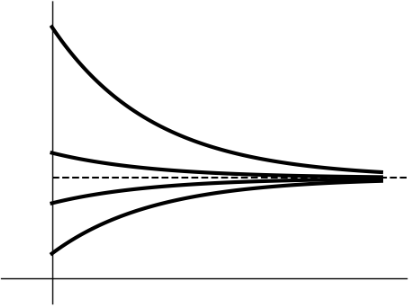
\includegraphics[width=0.8\textwidth]{coolingcurves}
\end{rightframe}


\begin{comment}
\begin{rightframe}[]
\begin{itemize}
    \item \textbf{Example}.  suppose we have a system with solution $s(t)$ which responds to an input $f(t)$:
        $$\dot s = -k s + f(t), \qquad s(0)=0$$
    
    suppose the input is pulses:
\end{itemize}

\vspace{5mm}
\includegraphics[width=0.8\textwidth]{pulsetrain}
\end{rightframe}


\begin{rightframe}[]
\begin{itemize}
    \item \textbf{Example}.  
        $$\dot s = -k s + f(t), \qquad s(0)=0$$
    
    the solution is
        $$s(t) = e^{-kt} \int_0^t e^{k\tau} f(\tau)\,d\tau$$
\end{itemize}

\vspace{5mm}
%\includegraphics[width=0.8\textwidth]{pulsetrain}
\end{rightframe}
\end{comment}


\begin{rightframe}[]
\begin{itemize}
    \item \textbf{Example}.
        $$x^2 y' + x(x+2) y = e^x$$
\end{itemize}
\end{rightframe}

\begin{rightframe}[]
\textbf{Expectations}

\bigskip
\begin{itemize}
\item \emph{read} section 2.3, including
  \begin{itemize}
  \item[*] an example with piece-wise functions
  \item[*] the error function as an example
  \end{itemize}
\item \emph{doing exercises} is essential
\end{itemize}
\end{rightframe}

\end{document}

